\documentclass[hidelinks]{report}
\usepackage{graphicx} % Required for inserting images
\usepackage{amsmath}
\usepackage{siunitx}
\usepackage{placeins}
\usepackage{tikz}
\usetikzlibrary{automata, arrows, positioning}
\usepackage{float}
\usepackage{hyperref}
\usepackage{cite}
\usepackage[utf8]{inputenc}
\usepackage[T1]{fontenc}
\usepackage{xcolor,graphicx}
\setcounter{secnumdepth}{0}
\usepackage{titlesec}
\usepackage[left=1.5in,top=1in,bottom=1in,right=1in]{geometry}
\usepackage{rotating}
\usepackage{subcaption}
\usepackage{lipsum}
\usepackage{fancyhdr}
\usepackage{mathptmx}
\usepackage{listings}
\usepackage{booktabs}
\usepackage{caption}
\usepackage{subcaption}
\usepackage{adjustbox}
\usepackage{enumitem}
\usepackage{setspace}
\usepackage{multirow}
\usepackage{amsmath}
\usepackage{algorithm}
\usepackage{algpseudocode}
\usepackage{tikz}
\setcounter{tocdepth}{4}
\usepackage{amsfonts}
\usepackage{fvextra}
\usepackage{minted}
\usepackage{xcolor}

\DefineVerbatimEnvironment{MyVerbatim}{Verbatim}{breaklines=true}
\usepackage{pgfplots}
\pgfplotsset{compat=1.17}
\newcommand{\mynote}[2]{\fbox{\bfseries\sffamily\scriptsize{#1}} {\small\textsf{\emph{#2}}}}

\newcommand{\hieplnc}[1]{\textcolor{red}{\mynote{hieplnc}{#1}}}

\newcommand{\sontg}[1]{\textcolor{blue}{\mynote{sontg}{#1}}}

\definecolor{blue}{RGB}{31,56,100}

\usepackage{lipsum}% http://ctan.org/pkg/lipsum
\makeatletter
\def\@makechapterhead#1{%
  {
  \parindent \z@ \raggedright \normalfont   
    
    \ifnum \c@secnumdepth >\m@ne
        \huge\bfseries \thechapter.\ % <-- Chapter # (without "Chapter")
    \fi
    \interlinepenalty\@M
    #1\par\nobreak% <------------------ Chapter title
    \vskip 40\p@% <------------------ Space between chapter title and first paragraph
  }}
\makeatother


% Redefine the \thesection and \thesubsection representations
\renewcommand{\thesection}{\arabic{chapter}.\arabic{section}}
\renewcommand{\thesubsection}{\thesection.\arabic{subsection}}
\renewcommand{\thesubsubsection}{\thesubsection.\arabic{subsubsection}}

% Define a new counter for subsections
\newcounter{subsecindex}[section]
\renewcommand{\thesubsecindex}{\thesubsection%
  \ifnum\value{subsecindex}>0
    .\arabic{subsecindex}%
  \fi
}

% Redefine the \section command to include the index
\let\oldsection\section
\renewcommand{\section}[1]{%
  \setcounter{subsecindex}{0} % Reset subsection counter for each section
  \refstepcounter{section}%
  \oldsection{\thesection\hspace{0.5em}#1}%
}

% Redefine the \subsection command to include the index
\let\oldsubsection\subsection
\renewcommand{\subsection}[1]{%
  \refstepcounter{subsection}%
  \oldsubsection{\thesubsecindex\hspace{0.5em}#1}%
}

% Redefine the \subsubsection command to include the index
\let\oldsubsubsection\subsubsection
\renewcommand{\subsubsection}[1]{%
  \refstepcounter{subsubsection}%
  \oldsubsubsection{\thesubsecindex\hspace{0.5em}#1}%
}

\titleformat{\section}
  {\normalfont\LARGE\bfseries} % Adjust \Large to any size you prefer
  {\thesection}{3em}{}
\titleformat{\subsection}
  {\normalfont\Large\bfseries} % Adjust \Large to any size you prefer
  {\thesubsection}{3em}{}
\titleformat{\subsubsection}
  {\normalfont\Large\bfseries} % Adjust \Large to any size you prefer
  {\thesubsubsection}{3em}{}
\lstset{
    language=Python,
    backgroundcolor=\color{gray!10},
    basicstyle=\ttfamily\small,
    keywordstyle=\color{blue},
    stringstyle=\color{orange},
    commentstyle=\color{gray},
    frame=single,
    showstringspaces=false
}
\begin{document}
\pagenumbering{gobble}

\pdfbookmark[0]{Main Title}{maintitle}
\begin{titlepage}
    \begin{tikzpicture}[remember picture,overlay,inner sep=0,outer sep=0]
        \draw[black!70!black,line width=1.5pt]
            ([xshift=-0.65in,yshift=-1cm]current page.north east) coordinate (A) -- % Adjusted x-shift and y-shift
            ([xshift=0.65in,yshift=-1cm]current page.north west) coordinate (B) -- % Adjusted x-shift and y-shift
            ([xshift=0.65in,yshift=1cm]current page.south west) coordinate (C) -- % Adjusted x-shift and y-shift
            ([xshift=-0.65in,yshift=1cm]current page.south east) -- % Adjusted x-shift
            cycle;
    \end{tikzpicture}

    \begin{center}
    \begin{figure}
        \centering
        \huge \uppercase{university of science and technology of hanoi} \\ [1.5 cm]
    
        \filleft
        \includegraphics[width=0.7\linewidth]{images/usth.png}
    \end{figure}
    
    \textsc{\Large }\\[1cm]
    {\huge \bfseries \uppercase{LABWORK'S REPORT}}\\[1cm]

    {\large \bfseries 2440053 - Dao Xuan Quy  } \\ [0.5cm]
    {\huge \bfseries \uppercase{Advance programming for HPC}}\\[1cm]
    
    % Title
    \rule{\linewidth}{0.3mm} \\[0.4cm]
    { \Huge \bfseries\color{blue}  Labwork 3: Hello, CUDA!}
    \rule{\linewidth}{0.3mm} \\[0.7cm]
    
    \large Academic Year: 2024-2026
    \end{center}

\end{titlepage}

\newpage
\pagenumbering{roman}
\noindent \Large \tableofcontents

\newpage
\listoffigures

\newpage
\listoftables

\thispagestyle{empty}
\newpage

\chapter{Introduction}
\pagenumbering{arabic}

\hspace{5mm} In this labwork I implements grayscale converter with 1D image with both CPUs and GPUs and compare the results. 
 
\chapter{Implementation \& Results}
\section{CPU grayscale}
For the CPU version, I simply use the \textbf{matplotlib} library for loading the image and \textbf{numpy} library for compress the image into 1D array images. 

Then, the formula to convert the RGB image into GrayScale Image is:

$gray\_pixel = \frac{red\_pixel + blue\_pixel + green\_pixel}{3}$

The full implementation could be seen in this code snipnet:
\begin{lstlisting}
    r = compressed_img[: ,0]
    g = compressed_img[: ,1]
    b = compressed_img[:, 2]
    gray_img = []
    for r_pixel, g_pixel, b_pixel in zip(r,g,b):
      gray_pixel = ((r_pixel + g_pixel +  b_pixel)/3)
      gray_img.append(gray_pixel)
\end{lstlisting}

The CPU takes 24.94 seconds to finish convert the image to grayscales. The result could be display as follow:
\begin{figure}[h!]
  \centering
  \begin{subfigure}[b]{0.45\textwidth}
    \centering
    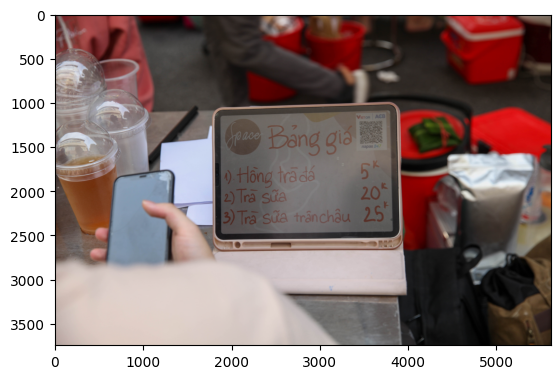
\includegraphics[width=\textwidth]{original.png}
    \caption{Original Image}
    \label{fig:og}
  \end{subfigure}
  \hfill
  \begin{subfigure}[b]{0.45\textwidth}
    \centering
    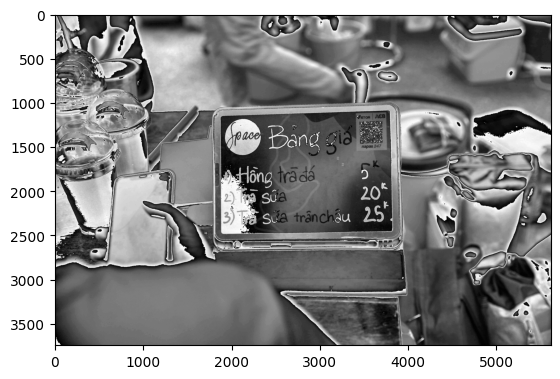
\includegraphics[width=\textwidth]{grayscale_cpu.png}
    \caption{Grayscale image (CPU)}
    \label{fig:cpu_gray}
  \end{subfigure}
  \caption{Grayscale conversion results}
  \label{fig:result_cpu}
\end{figure}

\section{GPU grayscale}
For GPU grayscale implementation, firstly, we need to define the CUDA JIT for grayscale conversion function:
\newpage
\begin{lstlisting}
    @cuda.jit
    def grayscale(src, dst):
      tidx = cuda.threadIdx.x + cuda.blockIdx.x * cuda.blockDim.x
      g = np.uint8((src[tidx, 0] + src[tidx, 1] + src[tidx, 2]) / 3)
      dst[tidx, 0] = dst[tidx, 1] = dst[tidx, 2] = g
\end{lstlisting}


Next, the image must be transfered from RAM to GPU's VRAM with \texttt{to\_device()} function. Also, to make computation faster, we also need to define the block size and grid size:

\begin{lstlisting}
    compressed_img_cuda = cuda.to_device(compressed_img)
    block_size = 64
    pixel_count = img.shape[0] * img.shape[1]
    grid_size = int(pixel_count/block_size)
\end{lstlisting}

Finally, execute the grayscale function as follow:

\begin{lstlisting}
    gray_img_cuda =  cuda.device_array((pixel_count, 1), dtype=np.uint8)
    grayscale[grid_size, block_size](compressed_img_cuda, gray_img_cuda)
    gray_img_host = gray_img_cuda.copy_to_host()
\end{lstlisting}

The image then is copied back to host for plotting. The conversion result could be seen in the figure \ref{fig:result_gpu} 
\begin{figure}[h!]
  \centering
  \begin{subfigure}[b]{0.45\textwidth}
    \centering
    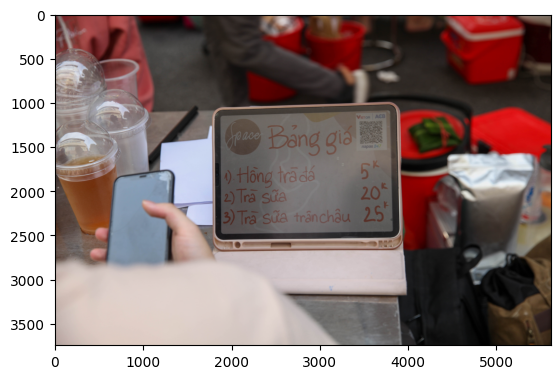
\includegraphics[width=\textwidth]{original.png}
    \caption{Original Image}
    \label{fig:og}
  \end{subfigure}
  \hfill
  \begin{subfigure}[b]{0.45\textwidth}
    \centering
    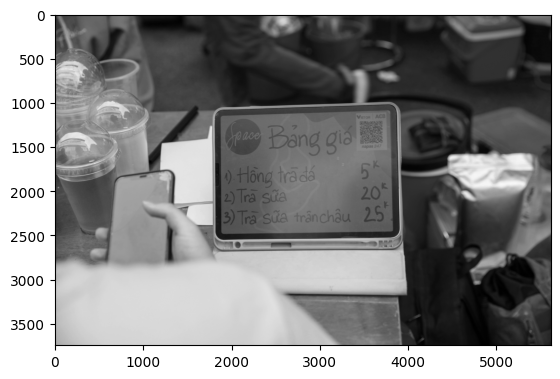
\includegraphics[width=\textwidth]{grayscale_gpu.png}
    \caption{Grayscale image (GPU)}
    \label{fig:cpu_gray}
  \end{subfigure}
  \caption{Grayscale conversion results}
  \label{fig:result_gpu}
\end{figure}

This time, it takes only 0.21 seconds to finish the code, while the CPU grayscale takes almost 30 seconds for the same task.

\newpage
\section{Evaluate Different block size}
With different block size, we could formulate a graph that illustates the behavior of the function (in runtime) when we increase the number of block size (figure \ref{fig:blocksize_runtime}):
\begin{figure}[h!]
    \centering
    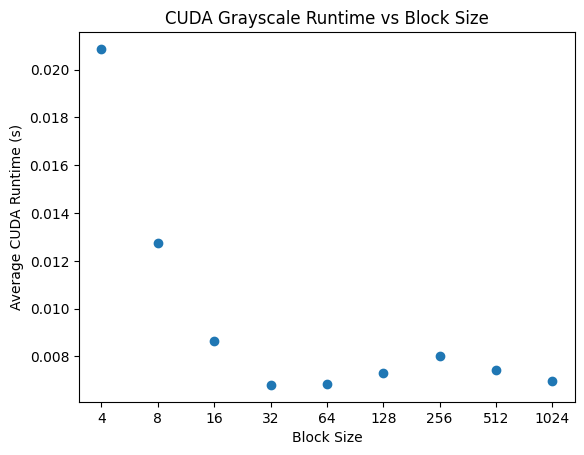
\includegraphics[width=0.7\linewidth]{blocksize_diff_graph.png}
    \caption{Blocksize vs Runtime}
    \label{fig:blocksize_runtime}
\end{figure}

Figure \ref{fig:blocksize_runtime} shows that with a larger blocksize, the function execute much faster (in a form of an exponential function)
\chapter{Conclusion}
In this lab, I implements grayscale converter algorithm for both CPU and GPU and witness the differences.
\end{document}